%
% sample project
%

%%%%%%%%%%%%%%%%%%%%%%%%%%%%%%%%%%%%%%%%%%%%%%%%%%%
% header 
%%%%%%%%%%%%%%%%%%%%%%%%%%%%%%%%%%%%%%%%%%%%%%%%%%%
\vspace{25pt}
\hrule
\section*{\bfsf Observational Cosmology Group} 
\vspace{12pt}
\hrule

\vspace{12pt}
\noindent
{\sf [Spokesperson : Yoshiaki Ono]}

\vspace{3pt}
\noindent
{\sf \small ICRR, The Univ. of Tokyo, Kashiwa, Chiba 277-8582}


\def\farcs{% 
 \mbox{% 
  \kern  0.13ex.% 
  \kern -0.95ex\raisebox{.9ex}{\scriptsize$\prime\prime$}% 
  \kern -0.1ex% 
 }% 
}

%\newcommand{\rqq}{\textquotedblright}
%\newcommand{\lqq}{\textquotedblleft}

%%%%%%%%%%%%%%%%%%%%%%%%%%%%%%%%%%%%%%%%%%%%%%%%%%%
% text 
%%%%%%%%%%%%%%%%%%%%%%%%%%%%%%%%%%%%%%%%%%%%%%%%%%%

\subsubsection*{\bi
SILVERRUSH. VIII. 
Spectroscopic Identifications of Early Large-scale Structures with Protoclusters 
over $200$ Mpc at $z\sim6$--$7$: 
Strong Associations of Dusty Star-forming Galaxies
{\rm \cite{harikane2019}}
}

\vspace{3pt}

\noindent
In collaboration with the members of 
\noindent
The University of Tokyo, 
National Astronomical Observatory of Japan, 
Aix Marseille University, 
Kitami Institute of Technology, 
California Institute of Technology, 
National Tsing Hua University, 
Osaka Sangyo University, 
Academia Sinica, 
University of California, Santa Barbara, 
Observatorio Nacional, 
Universidade de Sao Paulo, 
Durham University, 
RIKEN, 
Purple Mountain Observatory, 
Dalhousie University, 
Imperial College London, 
Seoul National University, 
Shanghai Jiao Tong University, 
Onomichi City University, 
Subaru Telescope, 
Nagoya University, 
Ehime University, 
and 
Cosmic Dawn Center. 

\vspace{10pt}

We have obtained three-dimensional maps of the universe 
in $\sim200\times200\times80$ comoving Mpc$^3$ (cMpc$^3$) volumes each at $z=5.7$ and $6.6$ 
based on a spectroscopic sample of 179 galaxies that achieves $\gtrsim80$\% completeness 
down to the Ly$\alpha$ luminosity of $\log(L_{\rm Ly\alpha}/[\mathrm{erg\ s^{-1}}])=43.0$, 
based on our Keck and Gemini observations and the literature 
(Figure \ref{cos:Harikane2019_Fig3}).
The maps reveal filamentary large-scale structures and two remarkable overdensities 
made out of at least 44 and 12 galaxies at $z=5.692$ (z57OD) and $z=6.585$ (z66OD), respectively, 
making z66OD the most distant overdensity spectroscopically confirmed to date, 
with $>10$ spectroscopically confirmed galaxies.
We compare spatial distributions of submillimeter galaxies at $z\simeq 4-6$ 
with our $z=5.7$ galaxies forming the large-scale structures, 
and detect a $99.97\%$ signal of cross-correlation, 
indicative of a clear coincidence of dusty star-forming galaxy and dust-unobscured galaxy formation 
at this early epoch.
The galaxies in z57OD and z66OD are actively forming stars with star-formation rates (SFRs) 
$\gtrsim5$ times higher than the main sequence, 
and particularly the SFR density (SFRD) in z57OD is 10 times higher than the cosmic average 
at the redshift (a.k.a. the Madau-Lilly plot).
Comparisons with numerical simulations suggest that 
z57OD and z66OD are protoclusters that are progenitors of the present-day clusters 
with halo masses of $\sim10^{14} M_\odot$.


%%%%%%%%%%%%%%%%%
% bibliography 
%%%%%%%%%%%%%%%%%

\begin{thebibliography}{9}
\bibitem[1]{harikane2019} 
Harikane, Y., Ouchi, M., Ono, Y., Fujimoto, S., Donevski, D., Shibuya, T., Faisst, A. L., Goto, T., Hatsukade, B., Kashikawa, N., Kohno, K., Hashimoto, T., Higuchi, R., Inoue, A. K., Lin, Y.-T., Martin, C. L., Overzier, R., Smail, I., Toshikawa, J., Umehata, H., Ao, Y., Chapman, S., Clements, D. L., Im, M., Jing, Y., Kawaguchi, T., Lee, C.-H., Lee, M. M., Lin, L., Matsuoka, Y., Marinello, M., Nagao, T., Onodera, M., Toft, S., Wang, W.-H. 
\ 2019, 
The Astrophysical Journal, 883, 142 
\end{thebibliography}


%--------------------------------------------------------------------------
\begin{figure}
\begin{center}
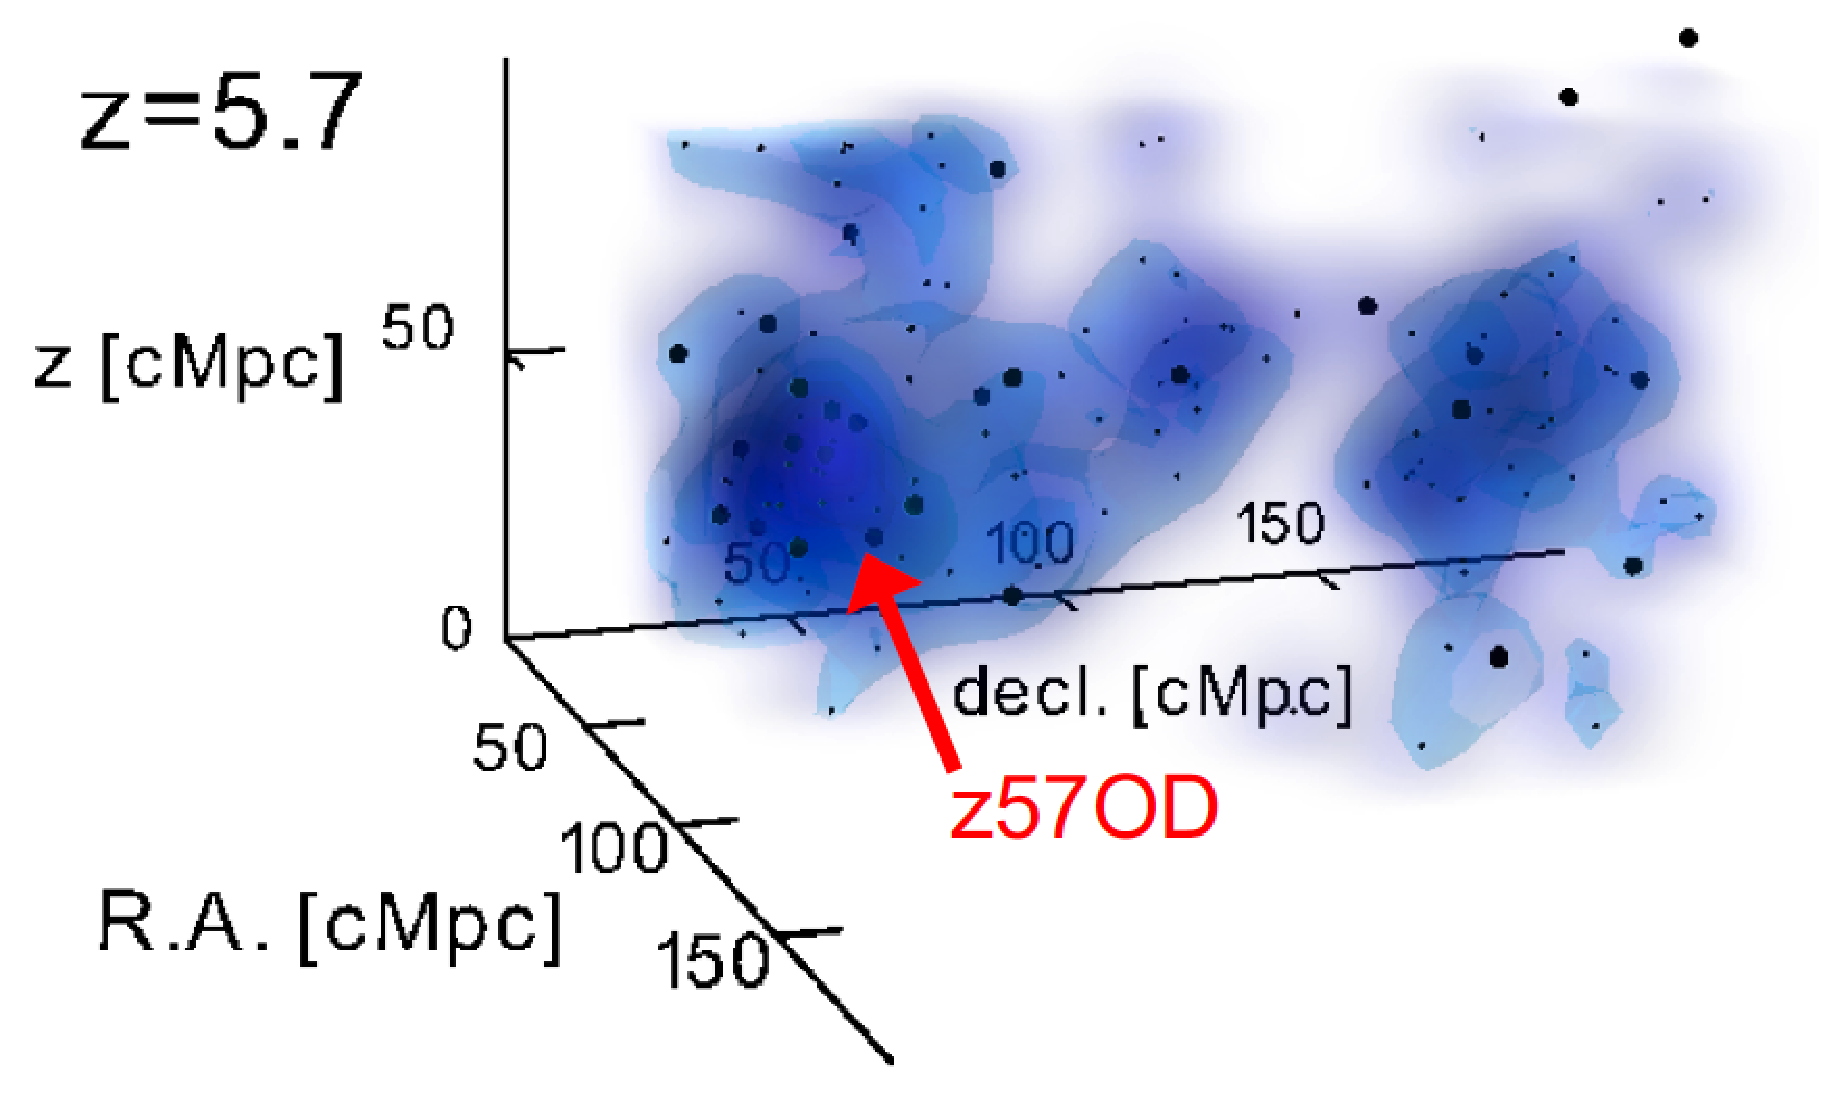
\includegraphics[height=4.7cm]{astrodiv/cos/Harikane2019_Fig3a.eps} 
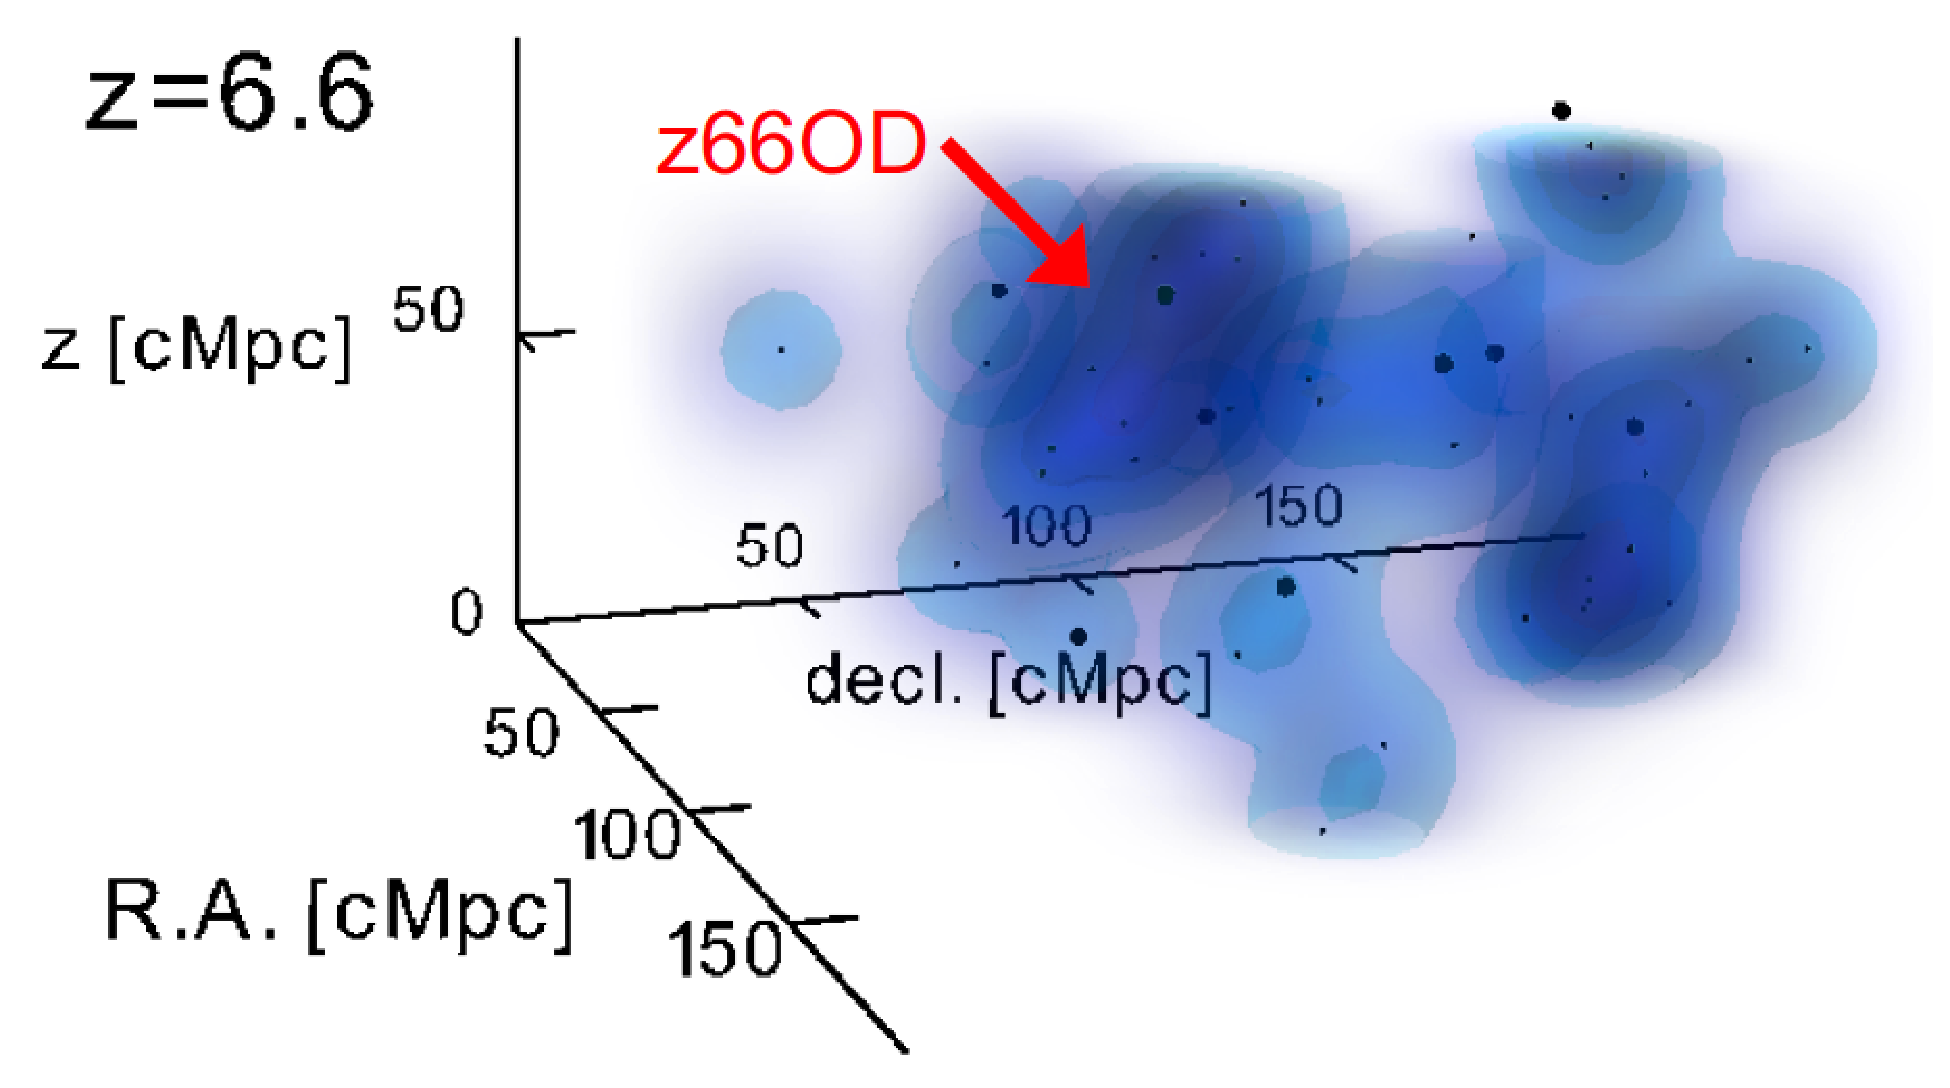
\includegraphics[height=4.7cm]{astrodiv/cos/Harikane2019_Fig3b.eps} 
\end{center}
\vspace{-5mm}
\caption{
3D overdensity maps of Ly$\alpha$ emitters (LAEs) at $z=5.7$ (top) and $z=6.6$ (bottom).
The black dots show the positions of the LAEs.
The large dots are LAEs brighter than $L_\mathrm{Ly\alpha}>10^{43}$ erg s$^{-1}$.
Higher density regions are indicated by the bluer colors, 
smoothed with a Gaussian kernel of $\sigma=10$ cMpc ($15$ cMpc) at $z=5.7$ ($z=6.6$).
}
\label{cos:Harikane2019_Fig3}
\end{figure}
%--------------------------------------------------------------------------






%%%%%%%%%%%%%%%%%%%%%%%%%%%%%%%%%%%%%%%%%%%%%%%%%%%
% text 
%%%%%%%%%%%%%%%%%%%%%%%%%%%%%%%%%%%%%%%%%%%%%%%%%%%

\subsubsection*{\bi
Fast Outflows Identified in Early Star-forming Galaxies at $z = 5$--$6$
{\rm \cite{sugahara2019}}
}

\vspace{3pt}

\noindent
In collaboration with the members of
\noindent
The University of Tokyo, 
National Astronomical Observatory of Japan, 
The University of Lyon, 
and 
Leiden Observatory. 

\vspace{10pt}

We present velocities of galactic outflows in seven star-forming galaxies at $z=5$--$6$ 
with stellar masses of $M_\ast \sim10^{10.1} M_\odot$. 
Although it is challenging to observationally determine the outflow velocities, 
we overcome this by using 
Atacama Large Millimeter/submillimeter Array (ALMA)
%ALMA 
[{\sc Cii}]158 $\mu$m emission lines for systemic velocities 
and deep Keck spectra with metal absorption lines for velocity profiles available to date. 
We construct a composite Keck spectrum of the galaxies at $z=5$--$6$ 
with the [{\sc Cii}]-systemic velocities, 
and fit outflow-line profiles to the Si{\sc ii}$\lambda1260$, C{\sc ii}$\lambda1335$, 
and Si{\sc iv}$\lambda\lambda1394,1403$ absorption lines in the composite spectrum. 
We measure the maximum (90\%) and central outflow velocities to be 
$v_{\rm max} = 700^{+180}_{-110}$ km s$^{-1}$ 
and $v_{\rm out} = 400^{+100}_{-150}$ km s$^{-1}$ on average, respectively, 
showing no significant differences between the outflow velocities 
derived with the low- to high-ionization absorption lines. 
For $M_\ast \sim10^{10.1} M_\odot$, 
we find that the $v_{\rm max}$ value of our $z=5$--$6$ galaxies is 3 times higher 
than those of $z\sim0$ galaxies and comparable to $z\sim2$ galaxies. 
Estimating the halo circular velocity $v_{\rm cir}$ from the stellar masses and the abundance matching results, 
we investigate a $v_{\rm max}$--$v_{\rm cir}$ relation (Figure \ref{cos:Sugahara2019_fig3}). 
Interestingly, $v_{\rm max}$ for galaxies with $M_\ast = 10^{10.0-10.8} M_\odot$ shows 
a clear positive correlation with $v_{\rm cir}$ and/or the galaxy star formation rate over $z=0$--$6$ 
with a small scatter of $\simeq \pm 0.1$ dex, 
which is in good agreement with theoretical predictions. 
This positive correlation suggests that the outflow velocity is physically related to the halo circular velocity, 
and that the redshift evolution of $v_{\rm max}$ at fixed $M_\ast$ 
is explained by the increase in $v_{\rm cir}$ toward high redshift.


%%%%%%%%%%%%%%%%%
% bibliography 
%%%%%%%%%%%%%%%%%

\begin{thebibliography}{9}
\bibitem[2]{sugahara2019} 
 Sugahara, Y., Ouchi, M., Harikane, Y., Bouch\'e, N., Mitchell, P. D., Blaizot, J. 
 \ 2019, 
The Astrophysical Journal, 886, 29 
\end{thebibliography}


%--------------------------------------------------------------------------
\begin{figure}
\begin{center}
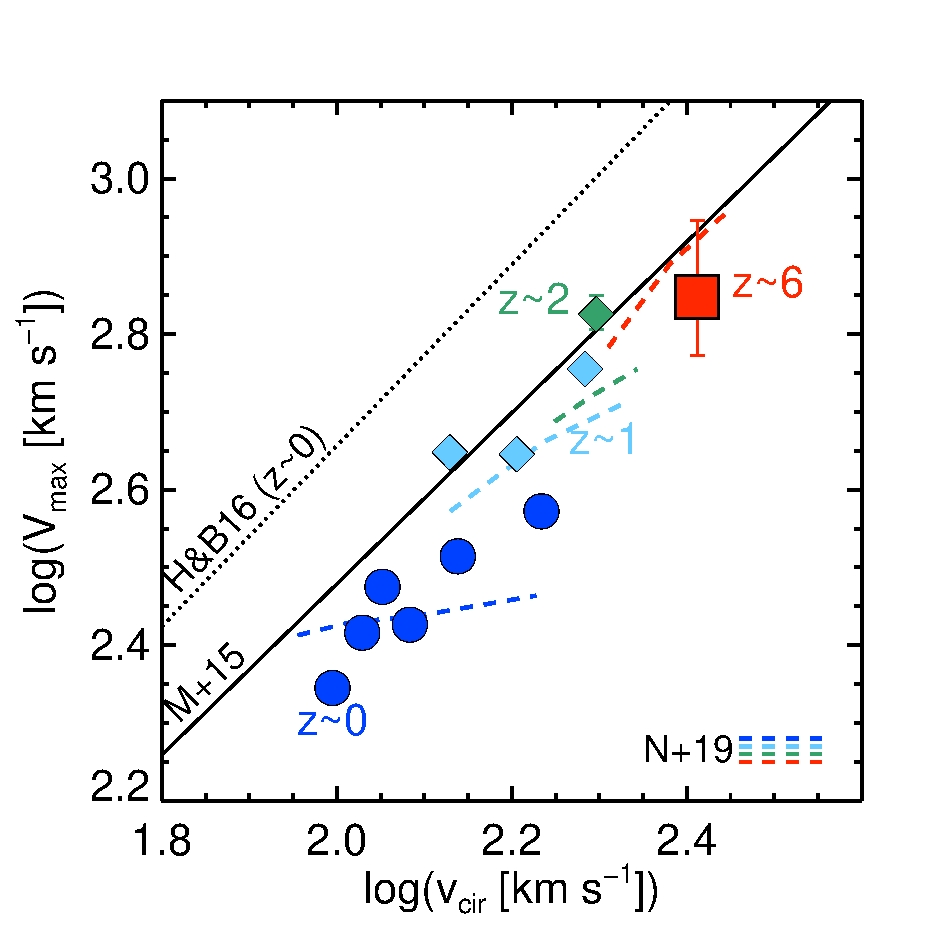
\includegraphics[width=8.5cm]{astrodiv/cos/Sugahara2019_Fig3.eps} 
\end{center}
\vspace{-5mm}
\caption{
$v_{\rm max}$ as a function of the circular velocity $v_{\rm cir}$ that are converted from the stellar mass. 
%The symbols are the same as in Figure \ref{fig:res1}. 
The filled red square indicates our results at $z=5$--$6$ 
measured with the simultaneous fitting of the Si{\sc ii} and {\sc Cii} lines. 
The data points at $z\sim0$ (blue) and $z\sim1$ (cyan) are 
taken from our previous work. 
%presented by Sugahara et al. (2017). 
The data point at $z\sim2$ is 
derived from the composite spectrum in our previous work, 
but re-calculated in the manner of this work
%The $v_{\rm max}$ value at $z\sim2$ (green) is 
%derived from the composite spectrum in Sugahara et al. (2017), but re-calculated in the manner of this work.
%
The solid, dashed, and dotted lines are obtained in the literature. 
The solid black line and colored dashed lines represent a theoretical relation at $z=0.5$--$4$ 
predicted by the FIRE simulations 
(the flux-weighted average 90th percentile velocity) 
%\citep[the flux-weighted average 90th percentile velocity;][]{Muratov:2015} 
and relations at $z=0$ (blue), $1$ (cyan), $2$ (green), and $6$ (red) 
predicted by the IllustrisTNG simulation 
(90th percentile velocity), 
%\citep[90th percentile velocity;][]{Nelson.D:2019a}, 
respectively. 
The dotted line indicates a relation of extreme-starburst galaxies $z\sim0$. 
%\citet{Heckman:2016}.
}
\label{cos:Sugahara2019_fig3}
\end{figure}
%--------------------------------------------------------------------------









%%%%%%%%%%%%%%%%%%%%%%%%%%%%%%%%%%%%%%%%%%%%%%%%%%%
% text 
%%%%%%%%%%%%%%%%%%%%%%%%%%%%%%%%%%%%%%%%%%%%%%%%%%%

\subsubsection*{\bi
First Identification of $10$ kpc [{\sc Cii}] $158\mu$m Halos around Star-forming Galaxies at $z = 5$--$7$ 
{\rm \cite{fujimoto2019}}
}

\vspace{3pt}

\noindent
In collaboration with the members of
\noindent
The University of Tokyo, 
National Astronomical Observatory of Japan, 
Waseda University, 
Scuola Normale Superiore, 
Centro Fermi, 
European Southern Observatory, 
University of Edinburgh, 
Osaka University, 
University of Tsukuba, 
and 
University of Nevada. 

\vspace{10pt}

We report the discovery of 10 kpc {\sc [Cii]} 158$\mu$m halos 
surrounding star-forming galaxies in the early Universe. 
We choose deep ALMA data of 18 galaxies, 
each with a star-formation rate of $\simeq 10$--$70\,M_\odot$ 
with no signature of 
%AGN
active galactic nucleus (AGN) 
whose {\sc [Cii]} lines are individually detected at $z=5.153$--$7.142$,
and we conduct stacking of the {\sc [Cii]} lines and dust continuum 
in the $uv$-visibility plane. 
The radial profiles of the surface brightnesses show a 10 kpc scale {\sc [Cii]} halo 
at the 9.2$\sigma$ level, significantly more extended than the 
\textit{Hubble Space Telescope} (HST) stellar continuum data
by a factor of $\sim5$ on the exponential-profile basis, as well as the dust continuum 
(Figure \ref{cos:fujimoto2019_fig11}).
We compare the radial profiles of {\sc [Cii]} and Ly$\alpha$ halos
universally found in star-forming galaxies at this epoch, 
and find that the scale lengths agree within $1\sigma$ level.
While two independent hydrodynamic zoom-in simulations match the dust and stellar continuum properties, 
the simulations cannot reproduce the extended {\sc [Cii]} line emission.
The existence of the extended {\sc [Cii]} halo is evidence of outflow remnants in the early galaxies 
and suggests that the outflows may be dominated by cold-mode outflows expelling the neutral gas. 

%%%%%%%%%%%%%%%%%
% bibliography 
%%%%%%%%%%%%%%%%%

\begin{thebibliography}{9}
\bibitem[3]{fujimoto2019} 
Fujimoto, S., Ouchi, M., Ferrara, A., Pallottini, A., Ivison, R. J., Behrens, C., Gallerani, S., Arata, S., Yajima, H., Nagamine, K. 
\ 2019, 
The Astrophysical Journal, 887, 107 
\end{thebibliography}


%--------------------------------------------------------------------------
\begin{figure*}
\begin{center}
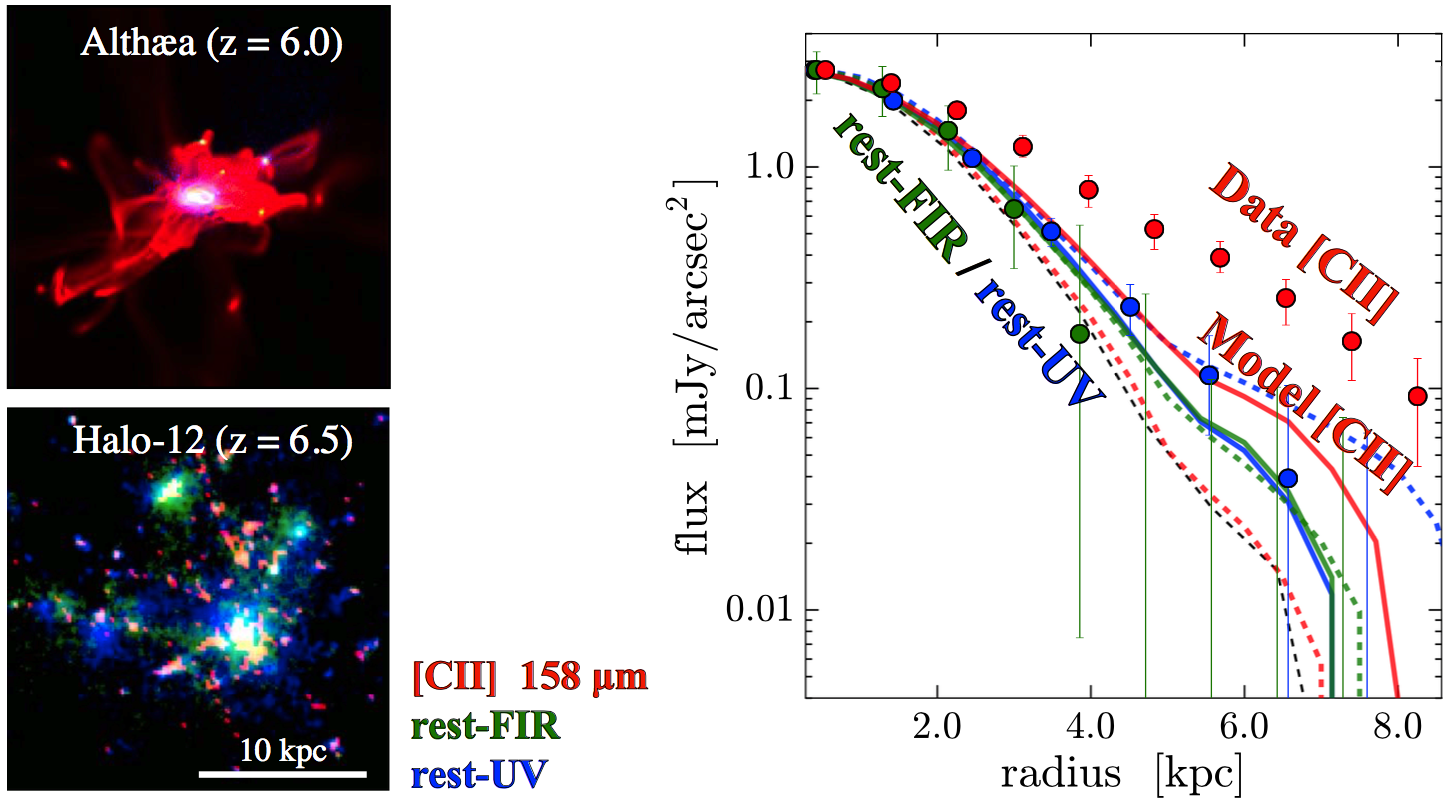
\includegraphics[width=16cm]{astrodiv/cos/Fujimoto2019_Fig11.eps} 
\end{center}
\vspace{-5mm}
\caption{
{\it \bf Left:} 
$4''\times4''$ fake-color image for Alth$\ae$a at $z=6.0$ (top) and Halo-12 (bottom) in the zoom-in simulations 
(red: {\sc [Cii]} line, green: rest-frame 
far-infrared (FIR)  
%FIR 
continuum, blue: rest-frame UV continuum). 
{\it \bf Right:} 
radial surface brightness profiles of the {\sc [Cii]} line (red curve), rest-frame FIR (green curve), and UV (blue curve) continuum emission estimated in the zoom-in simulations via a stacking procedure. 
The solid and dashed color lines represent the Alth$\ae$a and Halo-12 results, respectively.  
The black dashed curve denotes the ALMA synthesized beam. 
The circles indicate the ALMA-HST stacking results, whose colors are assigned in the same manner as the left panel.  
}
\label{cos:fujimoto2019_fig11}
\end{figure*}
%--------------------------------------------------------------------------






%%%%%%%%%%%%%%%%%%%%%%%%%%%%%%%%%%%%%%%%%%%%%%%%%%%
% text 
%%%%%%%%%%%%%%%%%%%%%%%%%%%%%%%%%%%%%%%%%%%%%%%%%%%

\subsubsection*{\bi
Balmer Break Galaxy Candidates at $z\sim6$: 
A Potential View on the Star Formation Activity at $z \gtrsim 14$ 
{\rm \cite{mawatari2020}}
}

\vspace{3pt}

\noindent
In collaboration with the members of
\noindent
Osaka Sangyo University, 
Waseda University, 
National Astronomical Observatory of Japan, 
University of Tsukuba, 
The University of Tokyo, 
Ehime University, 
Japan Aerospace Exploration Agency, 
Tohoku University, 
California Institute of Technology, 
Academia Sinica, 
and 
The Open University of Japan. 

\vspace{10pt}

We search for galaxies with a strong Balmer break (Balmer Break Galaxies; BBGs) 
at $z \sim 6$ over a 0.41\,deg$^2$ effective area in the COSMOS field. 
Based on rich imaging data, including data obtained with the ALMA, 
%Atacama Large Millimeter/submillimeter Array (ALMA), 
three candidates are identified by their extremely red $K - [3.6]$ colors, 
as well as by non-detection in X-ray, optical, 
%far-infrared (FIR), 
FIR, 
and radio bands. 
The non-detection in the deep ALMA observations suggests that 
they are not dusty galaxies but BBGs at $z \sim 6$, 
although contamination from 
%active galactic nuclei (AGNs) 
AGNs 
at $z \sim 0$ cannot be completely ruled out for the moment.
Our spectral energy distribution (SED) analyses reveal that 
the BBG candidates at $z \sim 6$ have stellar masses of $\approx 5 \times 10^{10}\,M_{\odot}$ 
dominated by old stellar populations with ages of $\gtrsim 700$ Myr. 
Assuming that all the three candidates are real BBGs at $z \sim 6$, 
we estimate the stellar mass density (SMD) to be $2.4^{+2.3}_{-1.3} \times 10^{4}\,M_{\odot}$\,Mpc$^{-3}$ 
(Figure \ref{cos:Mawatari2020_fig13}). 
This is consistent with an extrapolation from the lower-redshift measurements. 
The onset of star formation in the three BBG candidates is expected to be several hundred million years 
before the observed epoch of $z \sim 6$. 
We estimate the 
%star-formation rate density (SFRD) 
SFRD 
contributed by progenitors of the BBGs 
to be ($2.4$--$12) \times 10^{-5}\,M_{\odot}$\,yr$^{-1}\,$Mpc$^{-3}$ at $z > 14$ (99.7\% confidence range). 
Our result suggests a smooth evolution of the SFRD beyond $z = 8$. 

%%%%%%%%%%%%%%%%%
% bibliography 
%%%%%%%%%%%%%%%%%

\begin{thebibliography}{9}
\bibitem[4]{mawatari2020} 
Mawatari, K., Inoue, A. K., Hashimoto, T., Silverman, J., Kajisawa, M., Yamanaka, S., Yamada, T., Davidzon, I., Capak, P., Lin, L., Hsieh, B.-C., Taniguchi, Y., Tanaka, M., Ono, Y., Harikane, Y., Sugahara, Y., Fujimoto, S., Nagao, T. 
\ 2020, 
The Astrophysical Journal, 889, 137 
\end{thebibliography}



%--------------------------------------------------------------------------
\begin{figure}
\begin{center}
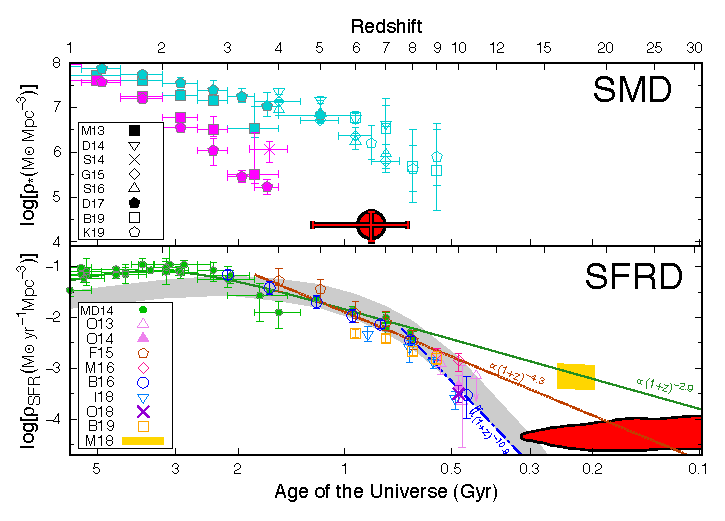
\includegraphics[width=8.5cm]{astrodiv/cos/Mawatari2020_Fig13.eps} 
\end{center}
\vspace{-5mm}
\caption{
Evolution of the SMD (top) and the SFRD (bottom) along the cosmic history (see top axis for the corresponding redshift). 
For these plots, we assume all the three BBG candidates without ALMA detection to be real passive galaxies at $z \sim 6$. 
In the top panel, the SMD of our BBG sample at $z \sim 6$ (red circle) is shown 
in conjunction with those of star-forming (cyan symbols) and passive (magenta symbols) galaxies at lower redshifts 
from the literature. 
%(M13: \citealt{Muzzin+13c}, D14: \citealt{Duncan+14}, S14: \citealt{Straatman+14}, G15: \citealt{Grazian+15}, S16: \citealt{Song+16}, D17: \citealt{Davidzon+17}, B19: \citealt{Bhatawdekar+19}, and K19: \citealt{Kikuchihara+19}). 
The vertical error bar associated with our BBG data corresponds to a $1\,\sigma$ uncertainty 
propagated from the Poisson error 
%\citep{Gehrels86} 
for the BBG number and the SED fitting uncertainty for the stellar mass. 
The horizontal error bar shows the redshift range expected from our BBG color selection. 
In the bottom panel, the red shaded region corresponds to the SFRD 
expected from the progenitors of the $z \sim 6$ BBGs at a $99.7$\,\% confidence level ($3\,\sigma$). 
The SFRD measurements at $z \lesssim 10$ are collected from the literature 
%(MD14: \citealt{Madau+14}, O13: \citealt{Oesch+13b}, O14: \citealt{Oesch+14}, F15: \citealt{Finkelstein+15a}, M16: \citealt{McLeod+16}, B16: \citealt{Bouwens+16c}, I18: \citealt{Ishigaki+18}, O18: \citealt{Oesch+18a}, and B19: \citealt{Bhatawdekar+19}). 
All of them at $4 \lesssim z \lesssim 10$ are estimated by integrating the UV 
luminosity functions 
%LFs 
down to $M_{\rm UV} = -17$\,mag. 
The SFRD estimated at $z \sim 17$ from an observed global 21\,cm absorption trough 
%(M18: \citealt{Madau18}, \citealt{Bowman+18}) 
is also shown in yellow. 
The functional fit to the MD14 data, which is proportional to $(1 + z)^{-2.9}$ at high-$z$,  
%\citep{Madau+14}, 
is superposed by the solid line. 
Two other power-law functions supporting an accelerated evolution at $z \gtrsim 8$ 
($\rho_{\rm SFR} \propto (1+z)^{-10.9}$)
%; \citealt{Oesch+14}) 
and a smooth evolution from lower redshift ($\rho_{\rm SFR} \propto (1+z)^{-4.3}$)
%; \citealt{Finkelstein+15a}) 
are shown by dotted-dashed and dotted lines, respectively. 
The SFRD derived assuming a universal relation among the halo mass, SFR, and dark matter accretion rate 
%\citep{Harikane+18a} 
is also superposed by the gray shade in its $1\,\sigma$ uncertainty. 
All of the SMD and SFRD measurements from the literature are corrected for the stellar IMF 
and the cosmological model to match those in this work. 
}
\label{cos:Mawatari2020_fig13}
\end{figure}
%--------------------------------------------------------------------------







%%%%%%%%%%%%%%%%%%%%%%%%%%%%%%%%%%%%%%%%%%%%%%%%%%%
% text 
%%%%%%%%%%%%%%%%%%%%%%%%%%%%%%%%%%%%%%%%%%%%%%%%%%%

\subsubsection*{\bi
CHORUS. III. Photometric and Spectroscopic Properties of Ly$\alpha$ Blobs at $z = 4.9$--$7.0$
{\rm \cite{zhang2020}}
}

\vspace{3pt}

\noindent
In collaboration with the members of
\noindent
The University of Tokyo, 
Kitami Institute of Technology, 
National Astronomical Observatory of Japan, 
Osaka Sangyo University, 
Waseda University, 
The Observatories of the Carnegie Institution for Science, 
University of Tsukuba, 
Osaka University, 
The Graduate University for Advanced Studies, 
Kure College, 
Observatoire de Geneve, 
Ehime University, 
and 
The Open University of Japan. 

\vspace{10pt}

We report the Subaru Hyper Suprime-Cam (HSC) discovery of two Ly$\alpha$ blobs (LABs), 
dubbed z70-1 and z49-1 at $z=6.965$ and $z=4.888$ respectively, 
that are Ly$\alpha$ emitters with a bright ($\log L_{\rm Ly\alpha}/{\rm [erg\ s^{-1}]}>43.4$) 
and spatially-extended Ly$\alpha$ emission, 
and present the photometric and spectroscopic properties of a total of seven LABs: 
the two new LABs and five previously known LABs at $z=5.7$--$6.6$. 
The z70-1 LAB shows extended Ly$\alpha$ emission with a scale length of $1.4\pm 0.2$ kpc, 
about three times larger than the UV continuum emission, 
making z70-1 the most distant LAB identified to date. 
All of the seven LABs, except z49-1, exhibit no AGN signatures such as X-ray emission, 
{\sc Nv}$\lambda$1240 emission, or Ly$\alpha$ line broadening, 
while z49-1 has a strong {\sc Civ}$\lambda$1548 emission line 
indicating an AGN on the basis of the UV-line ratio diagnostics. 
We carefully model the point-spread functions of the HSC images 
and conduct two-component exponential profile fitting 
to the extended Ly$\alpha$ emission of the LABs. 
The Ly$\alpha$ scale lengths of the core (star-forming region) 
and halo components are $r_{\rm c}=0.6$--$1.2$ kpc and $r_{\rm h}=2.0$--$13.8$ kpc, respectively. 
The relations between the scale lengths and galaxy properties 
(Ly$\alpha$ luminosity $L_{\rm Ly\alpha}$, Ly$\alpha$ rest-frame equivalent width EW$_0$, 
and UV continuum magnitude $M_{\rm UV}$) of our LABs 
are similar to those of Ly$\alpha$ halos (LAHs) 
identified around star-forming galaxies 
found previously by VLT/MUSE at similar redshifts (Figure \ref{cos:Zhang2020_Fig12}), 
suggesting that our LABs are likely the bright version of high-$z$ LAHs. 
%The average $r_{\rm h}$ of the LABs falls on the extrapolation of the $r_{\rm h}$-Ly$\alpha$ luminosity relation of the Ly$\alpha$ halos around VLT/MUSE star-forming galaxies at the similar redshifts, suggesting that typical LABs at $z\gtrsim5$ are not special objects, but star-forming galaxies at the bright end.

%%%%%%%%%%%%%%%%%
% bibliography 
%%%%%%%%%%%%%%%%%

\begin{thebibliography}{9}
\bibitem[5]{zhang2020} 
Zhang, H., Ouchi, M., Itoh, R., Shibuya, T., Ono, Y., Harikane, Y., Inoue, A. K., Rauch, M., Kikuchihara, S., Nakajima, K., Yajima, H., Arata, S., Abe, M., Iwata, I., Kashikawa, N., Kawanomoto, S., Kikuta, S., Kobayashi, M., Kusakabe, H., Mawatari, K., Nagao, T., Shimasaku, K., Taniguchi, Y.
\ 2020, 
The Astrophysical Journal, 891, 177 
\end{thebibliography}


%--------------------------------------------------------------------------
\begin{figure}
\begin{center}
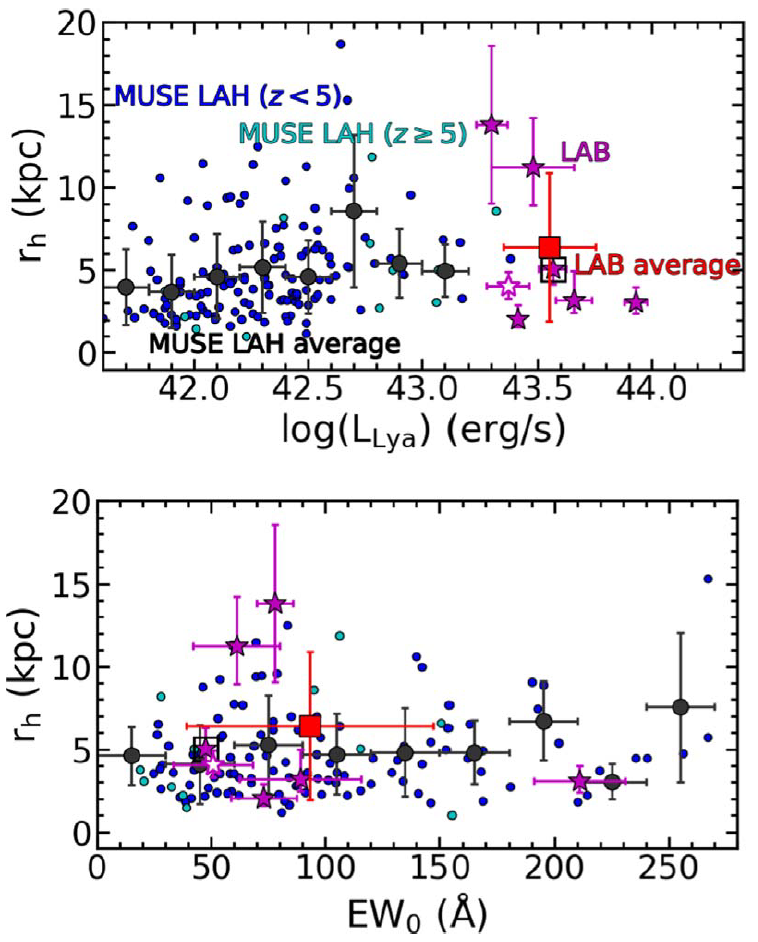
\includegraphics[width=8.5cm]{astrodiv/cos/Zhang2020_Fig12.eps} 
\end{center}
\vspace{-5mm}
\caption{
Halo scale length as a function of Ly$\alpha$ luminosity (top) and Ly$\alpha$ rest-frame equivalent width (bottom) 
of the seven LABs (stars) and LAHs (filled circles) from the literature. 
The empty star represents z57-2, which does not have a two-component fitting result. 
The red filled square shows the average value of our LABs, 
with error bars indicating the rms.  
The MUSE LAHs at $z<5$ and $z\geq5$ are the blue and cyan filled circles, respectively. 
The average values of the MUSE LAHs are shown as black filled circles. 
The black horizontal error bar indicates the bin size, 
while the black vertical error bar is the rms. 
%The solid lines represent the best-fit linear functions to the MUSE LAEs at $z=3-6$ (black) and $z=5-6$ (cyan), while the dashed lines are the extrapolations of the best-fit functions. It is clear that the average values of our LABs are consistent with the extrapolations of the best-fit functions of MUSE LAEs at $z=3-6$ and $z=5-6$. 
In the top panel, we slightly shift z49-1 (boxed star) along the horizontal axis by +0.03 to avoid overlaps.
}
\label{cos:Zhang2020_Fig12}
\end{figure}
%--------------------------------------------------------------------------



